\documentclass[a4paper]{article}
\title{Deep Learning}
\date{February, 2018}
\author{andrijazz}

\usepackage{hyperref}
\usepackage{amsmath}
\usepackage{graphicx}
%----------------------------------------------------------------------------------------

\usepackage{listings} % Required for inserting code snippets
\usepackage[usenames,dvipsnames]{color} % Required for specifying custom colors and referring to colors by name

\definecolor{DarkGreen}{rgb}{0.0,0.4,0.0} % Comment color
\definecolor{highlight}{RGB}{255,251,204} % Code highlight color

\lstdefinestyle{Style1}{ % Define a style for your code snippet, multiple definitions can be made if, for example, you wish to insert multiple code snippets using different programming languages into one document
	language=Python, % Detects keywords, comments, strings, functions, etc for the language specified
	backgroundcolor=\color{highlight}, % Set the background color for the snippet - useful for highlighting
	basicstyle=\footnotesize\ttfamily, % The default font size and style of the code
	breakatwhitespace=false, % If true, only allows line breaks at white space
	breaklines=true, % Automatic line breaking (prevents code from protruding outside the box)
	captionpos=b, % Sets the caption position: b for bottom; t for top
	commentstyle=\usefont{T1}{pcr}{m}{sl}\color{DarkGreen}, % Style of comments within the code - dark green courier font
	deletekeywords={}, % If you want to delete any keywords from the current language separate them by commas
	%escapeinside={\%}, % This allows you to escape to LaTeX using the character in the bracket
	firstnumber=1, % Line numbers begin at line 1
	frame=single, % Frame around the code box, value can be: none, leftline, topline, bottomline, lines, single, shadowbox
	frameround=tttt, % Rounds the corners of the frame for the top left, top right, bottom left and bottom right positions
	%keywordstyle=\color{Blue}\bf, % Functions are bold and blue
	morekeywords={}, % Add any functions no included by default here separated by commas
	numbers=left, % Location of line numbers, can take the values of: none, left, right
	numbersep=10pt, % Distance of line numbers from the code box
	numberstyle=\tiny\color{Gray}, % Style used for line numbers
	rulecolor=\color{black}, % Frame border color
	showstringspaces=false, % Don't put marks in string spaces
	showtabs=false, % Display tabs in the code as lines
	stepnumber=5, % The step distance between line numbers, i.e. how often will lines be numbered
	stringstyle=\color{Black}, % Strings are purple
	tabsize=2, % Number of spaces per tab in the code
}

% Create a command to cleanly insert a snippet with the style above anywhere in the document
\newcommand{\insertcode}[2]{\begin{itemize}\item[]\lstinputlisting[caption=#2,label=#1,style=Style1]{#1}\end{itemize}} % The first argument is the script location/filename and the second is a caption for the listing

%----------------------------------------------------------------------------------------

\begin{document}
\maketitle

%\insertcode{"SetupEC2ForTorch.txt"}{Setting up server for deep learning in Torch.}

\section{Introduction to Deep Learning}
Andrew Ng is introducing $ReLU$ (Rectified Linear Unit) function which is often seen in deep learning literature as an example of the simplest choice for activation function. 
\begin{align}
f(x) =
	\begin{cases}
		x   & \quad x \geq 0\\
		0	& \quad x < 0
	\end{cases}
\end{align}

\begin{figure}[!h]
	\centering
	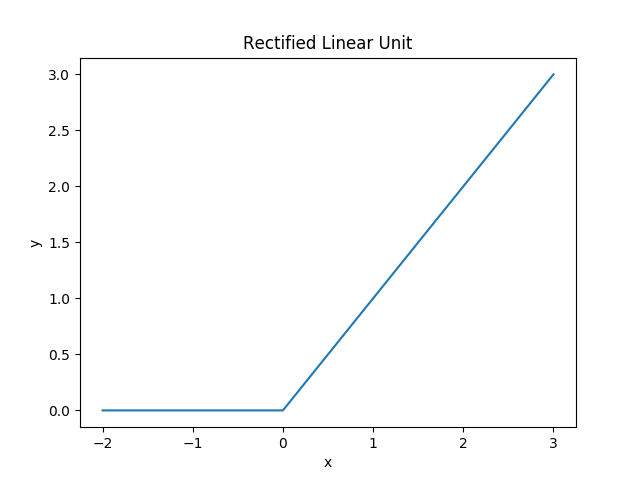
\includegraphics[width=50mm]{../plots/relu.png}
	\caption{ReLU function}
	\label{fig:relu}
\end{figure}

One of the major breakthroughs in NN computations was introducing $ReLU$ function instead of $Sigmoid$ function $f(x) = \frac{1}{1 + e ^{-x}}$. The advantage of $ReLU$ is that has value $0$ when $x < 0$, where $Sigmoid$ function has values that are close to $0$ and thus making the computation harder.
Additionally, gradient of $ReLU$ function is equal to $1$ for all positive $x$'s and thus making the gradient descent runs much faster.

Especially interesting in Week 1 of the course was interview with Geoffry Hinton where a lot of interesting ideas were mentioned so it would be really beneficial to watch this video again once student gain more knowledge about different models like Boltzman Machines etc.

\section{Neural Network Basics}

\subsection{Image representation}
Image is represented with the 3-dimensional matrix where dimensions represent values of Red Green and Blue respectively. 3-dimensional matrix is usually squeezed into 1-dimensional vector and this is what we are considering to be our $x$ in terms of image classification models.

\subsection{Binary classification and Neural Network Notation}
In this section Andrew Ng defines binary classification problem, introduces Logistic Regression and $Sigmoid$ function but more importantly it introduces neural network notation that will be used throughout the course. He emphasizes that neural network notation will be different from the one used in his first Machine Learning course in a way that bias will be kept separately of parameters vector because it is more natural notation when implementing neural net.

For detail notation take a look at the file \textit{neuralnetworknotation.pdf}.

\subsection{Logistic regression cost function}
We define a \textbf{loss function} as a measurement of how well we are doing on a single training example and \textbf{cost function} of how well we are doing on the entire training set.

Loss function for Logistic regression is:

\begin{align}
L(y, \hat{y}) = -(y\log{\hat{y}} + (1 - y)\log{(1 - \hat{y})})
\end{align}

where $\hat{y} = \sigma(w^Tx + b)$ and $\sigma$ is $Sigmoid$ function.
The questions that pops up is why we simply can't use $L(y, \hat{y}) = \frac{1}{2}(y - \hat{y})$ as a loss function? The answer is that optimization problem that we will encounter will become non-convex and thus gradient descent may converge to local optimum instead of global optimum.

Cost function for Logistic regression is:
\begin{align}
J(W, b) = \frac{1}{m}\sum_{i = 1}^{m}(L(y^{(i)}, \hat{y}^{(i)}) = -\frac{1}{m}\sum_{i = 1}^{m}(y^{(i)}\log{\hat{y}^{(i)}} + (1 - y^{(i)})\log{(1 - \hat{y}^{(i)})})
\end{align}

People usually don't do random initialization for Logistic Regression because cost function is convex and thus the usual way is to simply initialize all the parameters to $0$.
\end{document}
